% Chapter 1

\chapter{Introduction} % Main chapter title

\label{Chapter1} % For referencing the chapter elsewhere, use \ref{Chapter1} 

\lhead{Chapter 1. \emph{Introduction}} % This is for the header on each page - perhaps a shortened title

%----------------------------------------------------------------------------------------
%\DeclareMathOperator*{\Min}{Min}
The problem addressed is to find a local minimizer of the nonsmooth minimization problem

\begin{equation} \label{mainproblem}
  \begin{aligned}
    & \underset{x \in \mathbb{R}^n}{\text{min}}
    & & f(x) \\
    & \text{s.t.}
    & & l_i \leq x_i \leq u_i , \; \\
    & & & i = 1, \ldots, n.
  \end{aligned}
\end{equation}

where $f \colon \mathbb{R}^n \to \mathbb{R}$, is continuous but not differentiable everywhere and $n$ is a very large but finite number.

The $L-BFGS-B$ algorithm \citep{lbfgsboriginal} is a standard method for solving large instances of \ref{mainproblem} when $f$ is a smooth function. The original name of $BFGS$ stands for Broyden, Fletcher, Goldfarb and Shanno, the authors
of the original "BFGS" quasi-Newton algorithm for unconstrained
optimization discovered and published
independently by them in 1970 [give the 4 references here].
This method requires storing and updating a matrix which 
approximates the inverse of the Hessian matrix $\nabla^2 f(x)$ and
hence requires $\mathcal{O}(n^2)$ operations per iteration.  
The $L-BFGS$ variant [give reference] is based on BFGS
but requires only $\mathcal{O}(mn)$ operations per iteration: thus,
the L stands for Large.  Finally, the last letter B in 
$L-BFGS-B$ stands for bounds, meaning the lower and upper
bounds $l_i$ and $u_i$ in \ref{mainproblem}.  $The L-BFGS-B$ algorithm
is implemented in a well known $FORTRAN$ software package
by the same name [give reference].

In this thesis, there is a brief description of the $L-BFGS-B$ algorithm
at a high level and then explain how the modified algorithm
is more suitable for functions $f$ which may not be
differentiable at their local or global optimizers.  
We call the new algorithm L-BFGS-B-NS where NS stands for
Non-Smooth.  We implemented these changes in a modified version 
of the Fortran code [ref] which is can be downloaded from the website
for this thesis [give URL].  We report on some numerical experiments 
that strongly suggest that the new code should be useful for the
nonsmooth bound-constrained optimization problem (1.1).

We are grateful to Jorge Nocedal and his coauthors for allowing us 
to modify the L-BFGS-B code and post the modified version.  

%\chapter{deleted chapter}

%Larger problems not only mean that their solution will take a longer time to solve. But storing and calculating a the necessary matrices depends on the capabilities of the machine used to solve the problem and this might be prohibitively expensive. There a few large scale optimization techniques that have already been developed for the case when $n$ is very large. Also, several techniques have already been developed to handle this type of problems as long as the function $f$ is smooth. But there is not much out there about large scale problems with nonsmooth $f$

%In this thesis $f(x)$ is a nonsmooth function. This small change will require a few changes in the solution algorithm.

%For the particular case when $n$ is a small number, several methods that solve optimization problems of nondifferentiable functions in lower dimensions \citep{kiwiel85} have been developed. This thesis will try to see if it is possible to bring some of those concepts to large scale optimization. 

%In the case of smooth functions, it is possible to use Newton iteration algorithms and achieve quadratic convergence, the problem with Newton algorithms is that they require second derivatives to be provided\footnote{the main issue with the second derivative is that it requires a total of $n \times n$ partial derivatives. Which is impractical for medium and for some small-size problems}. In the 1950's and several years after that, several "quasi-newton" methods were proposed where the second derivative Hessian matrix is approximated step by step \citep{unconstrained}. These approximations or "updates" are calculated after every iteration of the original algorithm and the way in which this update is found defines a new method depending on the particular needs. This thesis will only be concerned with the $BFGS$. \footnote{BFGS stands for the last names of its authors Broyden, Fletcher, Goldfarb and Shanno} which can achieve super linear convergence, has proven to work in most practical purposes and posseses very nice self correcting features \citep{selfcorrecting}. In $BFGS$, it doesn't matter that one update incorrectly estimates the curvature in the objective function, $BFGS$ will always correct itself in just a few steps. This self-correcting property is very desired in the nonsmooth case, since changes in curvature could be abrupt near the optimal point. 

%$BFGS$ was originally developed for small to medium sized problems, and it is not the right tool for large scale optimization and therefore an $L-BFGS$ adaptation is needed to solve large scale problems\ref{mainproblem}. 

%A final assumption in this thesis is that the Hessian matrix is not sparse. In this case, there are other algorithms that may be more suitable \citep{Fletcher96computingsparse, sparse}, some of them have even been implemented in fortran \citep{lancelot}.

%This thesis builds upon the original $L-BFGS-B$ code \citep{lbfgsbsoftware} that solves smooth problems of $f$. There were three main changes in the code. The first one is the line search descent and curvature conditions which required a weaker version of the curvature in order to satisfy the different structure that a nonsmooth function requires. The second one is the line search methodology which was changed from a cubic interpolation to a bisection algorithm and last change in the thesis was the termination condition.

%Nocedal's original algorithm consists of $2$ steps. In the first step or gradient projection, most of the dimensions in the problem should be removed, making the problem a lot simpler. In the second step there is some fine tuning to guarantee better than just linear speed of convergence.

\chapter{L-BFGS-B}
\label{ChapterConstraints} % For referencing the chapter elsewhere, use \ref{ChapterConstraints} 

This section is a description of the original $L-BFGS-B$ code at a very high level \citep{lbfgsbsoftware}. The original software is intended to work well with smooth functions. This thesis discusses how to modify the algorithm for Non-Smooth functions.

\section{BFGS}

$BFGS$ is a standard tool for optimization of smooth functions. It is a line search method and its goal is to find a search direction starting from its current position $x$. The search direction is of type $d = -B \nabla f$ \footnote{Notice that when $B$ is the identity, this is the same direction as steepest descent. Another common line search method of optimization} where $B$ is an approximation to the inverse Hessian. \footnote{When it is exactly the inverse Hessian the method is known as Newton's method. Newton's method has quadratic convergence but requires the explicit calculation of the Hessian at every single step.} This $k^{th}$ step approximation is calculated via the $BFGS$ formula

\begin{equation} \label{bfgsupdate}
  \begin{aligned}
    B_{k+1} = \left(I - \frac{s_ky_k^T}{y_k^Ts_k} B_{k} \left( I - \frac{y_ks_k^T}{y_k^Ts_k} \right) + \frac{s_k s_k^T}{y_k^T s_k}\right)
  \end{aligned}
\end{equation}

where $y_k = \nabla f(x_{k+1}) - \nabla f(x_k)$ and $s_k = x_{k+1} - x_k$ and where the first approximation of $B_0$ is assumed to be the the identity matrix $I$ in this thesis.  $BFGS$ exhibits superlinear convergence but it also requires $\mathcal{O}(n^2)$ operations per iteration. \citep{nocedal}

In the case of Non-Smooth functions. $BFGS$ typically succeeds in finding a local minimizer. This is partly because $BFGS$ has some nice self-correcting properties, however this requires some modifications of the line search conditions. This change to the line search conditions is known as the weak Wolfe line search and it will be explained later in this thesis.

\section{L-BFGS}

$L-BFGS$ stands for Limited-memory $BFGS$. This algorithm approximates $BFGS$ using only a limited amout of computer memory to approximate the inverse of the Hessian $B$. So Instead of storing a dense $n \times n$ matrix, $L-BFGS$ keeps a record of the last $m$ iterations where $m$ is a small number that is chosen according to the problem at hand. \footnote{In this thesis $m < 20$, and in practice numbers between 5 and 10 are regularly used. There is no way of knowing a priori what choice of $m$ will provide the best results} It is for this reason that during the first $m$ iterations, $BFGS$ and $L-BFGS$ produce exactly the same search directions.

Because of this construction, the $L-BFGS$ algorithm is less computationally intensive and it only requires $\mathcal{O}(mn)$ iterations. So it is much better suited for problems where the number of dimensions $n$ is large. For this reason it is the algorithm of choice in this thesis.

\section{L-BFGS-B}

Finally $L-BFGS-B$ comes naturally as an extension of $L-BFGS$. The $B$ stands for the inclusion of Boundaries.  $L-BFGS-B$ requires two extra steps on top of $L-BFGS$. First, a gradient projection that reduces the dimensionality of the problem. Depending on the problem, the gradient projection could potentially save a lot of iterations by eliminating those variables that are at bound at the optimum. After that, the subspace minimization; here, during the search step phase the step length is restricted as much as necessary in order to remain within the box defined by \ref{mainproblem}.

\subsection{Gradient Projection}
The original algorithm was created for the case when $n$ is large and $f$ is smooth. Its first step is a gradient projection similar to the one outlined in \citep{gradproj1, gradproj2} which is used to determine an active set corresponding to those variables that are on either their lower or upper bounds. The active set defined at point $x^*$ is:

\begin{equation}
  \begin{aligned}
    \mathcal{A}(x^*) = \{ i \in \{1 \ldots n\} |  x^*_i = l_i \vee  x^*_i = u_i\}
  \end{aligned}
\end{equation}

Working with this active set is efficient in large scale problems. A pure line search algorithm would have to choose a step length short enough to remain within the box defined by $u_i$ and $l_i$. So if at the optimum, a large number $\mathcal{B}$ of variables are either on the lower or the upper bound. At least a number $\mathcal{B}$ of iterations might be needed. Gradient projection tries to reduce this number of iterations. In the best case, only $1$ iteration is needed instead of $\mathcal{B}$.

Gradient projection works on the approximation model:

\begin{equation} \label{themodel}
  \begin{aligned}
    m_k(x) = f(x_k) + \nabla f(x_k)^T ( x - x_k) + \frac{(x - x_k)^T H_k (x - x_k) }{2}
  \end{aligned}
\end{equation}

where $H_k$ is a $L-BFGS-B$ approximation to the Hessian $\nabla^2 f$ stored in the implicit way defined by $L-BFGS$.

In this first stage of the algorithm a piecewise linear segment starts on the current point $x_k$ in the direction $-\nabla f(x_k)$. Whenever this direction encounters one of the constraints, the line segment turns corners in order to remain feasible. The path is nothing but the feasible piecewise projection of the negative gradient direction on the constraint box determined by the values $\overrightarrow{l}$ and $\overrightarrow{u}$. At the end of this stage, the value of $x$ that minimizes $m_k(x)$ restricted to this piecewise gradient projection path is known as the 'Cauchy point' $x^c$.

\subsection{Subspace Minimization}

The problem with gradient projection is that its search direction does not take advantage of information provided implicitly by $H_k$, and therefore the speed of convergence is at best linear. It is for this reason that a stage two is necessary. Stage 2 or subspace minimization uses an $L-BFGS$ implicit approximation of the Inverse Hessian matrix restricted to the free variables that are not in the active set $\mathcal{A}(x^c)$.

The idea at a higher level is to solve the constrained problem \ref{themodel}, but only on those dimensions that are free. The starting point for this new problem will be the previously found Cauchy point $x^c$, the $L-BFGS$ approximation will provide a new search direction $\hat{d}^u$ that takes implicit advantage of second order approximations of the Hessian matrix.

The algorithm will move in the direction $\hat{d}^* = \alpha^* \hat{d}^u$ where $\alpha^*$ (the step length) is chosen so that the new point $\bar{x}_i$ satisfies weak wolfe descent and curvature conditions, A third restriction on the step length is added so that the next iteration stays feasible. Once this step is finished, the next and final step will be the termination condition. If the termination condition fails a new gradient projection and subspace minimization will be needed.

\chapter{Modifications to the L-BFGS-B algorithm}

As it was mentioned earlier there were three main changes in the original code by Nocedal\citep{lbfgsbsoftware}. They were the line search Wolfe conditions, the line search methodology, and the termination condition.

\section{The Wolfe conditions}

Probably the most important change made to the original code was the change in the curvature condition. Originally there are two Wolfe conditions, one of them is the Armijo condition, also known as the sufficient decrease requirement. The other one is the curvature condition, of which the most popular version is the strong wolfe curvature condition:

\begin{equation}
  \begin{aligned}
    |p_k^T \nabla f(x_k + \alpha _k p_k)| \leq |p_k^T \nabla f(x_k)|
  \end{aligned}
\end{equation}

The strong wolfe is a more natural way to see and achieve convergence, but the problem is that it does not work well for the nonsmooth case. This is because near the minimal points, there may be abrupt changes in curvature. In these cases there is no other option but to relax the curvature condition as long as the sufficient decrease condition is satisfied. The suggested new decrease condition is this one:

\begin{equation}
  \begin{aligned}
    p_k^T \nabla f(x_k + \alpha _k p_k) \geq p_k^T \nabla f(x_k)
  \end{aligned}
\end{equation}

It is noticeable that with this new condition the algorithm does not crash in the problems tested, as opposed to when the hard wolfe condition is used.

\section{The line search}

The original software by Nocedal\citep{lbfgsbsoftware}, included a cubic line search. The idea of a cubic interpolation line search is to take advantage of the smooth properties of function $f$ in order to find a more convenient point. But in the case of nonsmooth functions, this line search does not serve our purposes and therefore a more typical line search that implements a bisection has to be used.

In general, a step length is selected. If this step length does not satisfy the sufficient decrease and curvature conditions then a step length of half or double the size is selected. the algorithm is guaranteed to converge under a careful selection of the parameters. However, in case this does not happen, the software will stop with a warning.

\section{The termination condition}

The most important requirement of a practical algorithm is that it ends in a finite time. For the case of smooth functions, the formal way to check whether the algorithm has finished, is to check whether the projected gradient has norm zero $0$ wherever the constraints are not at bound. In the case of nonsmooth functions however, this is not necessarily true and the function at the minimum, may have a kink. In this kink the projected gradient may not vanish. Furthermore, if there is a sequence of points that approaches the optimum $x$ from the right, the projected gradients corresponding to this sequence of points might be completely different from the projected gradients associated to a sequence of points that approach the optimum $x$ from the left.

Given this set of conditions, there is the need for a special set of rules to establish the finalization of each optimization.

Since BFGS approximations typically converge to Clarke-Stationary points. The right methodology should be to calculate the subgradient and to see wheter zero $0$ is part of this subgradient. One particular methodology that guarantees an end to the algorithm is suggested in \citep{overtonlewis}. In order to make sure that the gradient zero $\vec{0}$ is part of the subgradient calculated over a neighbourhood of the optimum. The algorithm keeps a record of the latest gradient vectors in a small neighbourhood of the point where it suspect that the optimum is located. This collection of gradients spans an associated convex hull of gradients. If this convex hull contains at least one vector of norm smaller than a small number $\tau_k$, the algorithm ends.

Of course the best way to find a vector with such properties is to find the vector with the minimal norm that resides in the convex hull.

\subsection{The Solution of the quadratic program}

The termination condition is guaranteed to end up at a local optimum. However in order to find the vector with the minimal norm one subalgorithm needs to be solved. This subalgorithm is a practical primal-dual algorithm implemented in \citep{skaaja}. In this case in particular the best solution is to implement a variation of Mehrotra's Predictor-Corrector algorithm applied to quadratic programming. The primal dual method requires the solution of a system in order to calculate the search direction. The most expensive part of this solution is the calculation of the cholesky decomposition. Mehrotra's algorithm uses the same cholesky decomposition to calculate both directions. the predictor, and the corrector.

Currently there is not a theoretical calculation of the complexity of this algorithm but it is widely used in practice with great results. The implementation on \citep{skaaja} is is exactly the one on \citep{nocedal}. In this thesis it was implemented in $FORTRAN$ as part of the optimizer.

\chapter{the solution test functions}

In order to make some tests, a few functions will be evaluated. The most important function to test this non-smooth optimizer is a modified version of rosenbrock's:

\begin{equation}
    f(x) = (x_1 - 1)^2 + \sum_{i = 2}^n |x_i - x_{i - 1}^2|^p
\end{equation}

Where the value of $p$ changes the behaviour of the optimizer. This function can be proven to be lipschitz continuous whenever $p > 1$ if restricted to the domain defined by  

\begin{equation}
  \begin{aligned}
    x_i = 
    \begin{cases}
      [-100, 100] & \text{if } i \in \text{ even numbers} \\
      [10, 100] & \text{if } i \in \text{ odd numbers}
    \end{cases}
  \end{aligned}
\end{equation}

and in fact, whenever the function is restricted to a finite domain this function will be lipschitz continuous for $p > 1$. Whenever $p > 1$ the function $f(z) = |z|^p$ is zero $0$ around zero because the derivative $p |z| ^{p-1}$ is zero whenever $z$ tends to zero from the right. (this is also the case from the left because it is an even function). However the second derivative will not be as nice.

For the case when $p \leq 1$ the second derivative tends to infinity. $\displaystyle \lim_{x \to 0^+} {f' = \infty}$. Which is already well known given the "heavyside" look of $f(z) = |z|$.

The convergence of the algorithm smoothly descends to the objective 

\begin{center}
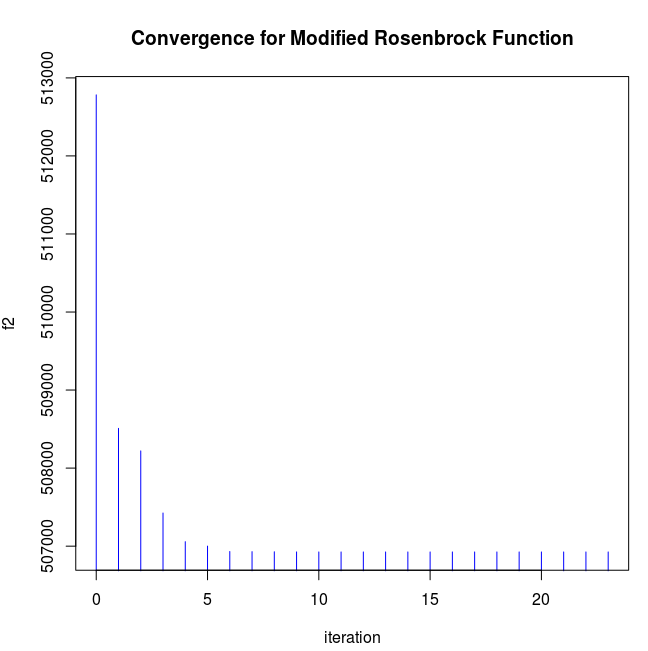
\includegraphics[scale=0.3]{Figures/convergence.png}
\end{center}

The converge is adversely affected by the selection of $p$ as one would expect. Values of $p$ descending to $1$ make the function less "smooth" and have the adverse effect of making the convergence much more difficult. In this exercise it is noticeable how slow the convergence becomes for a few specific values of $p$. In particular for $1.0001$

\begin{center}
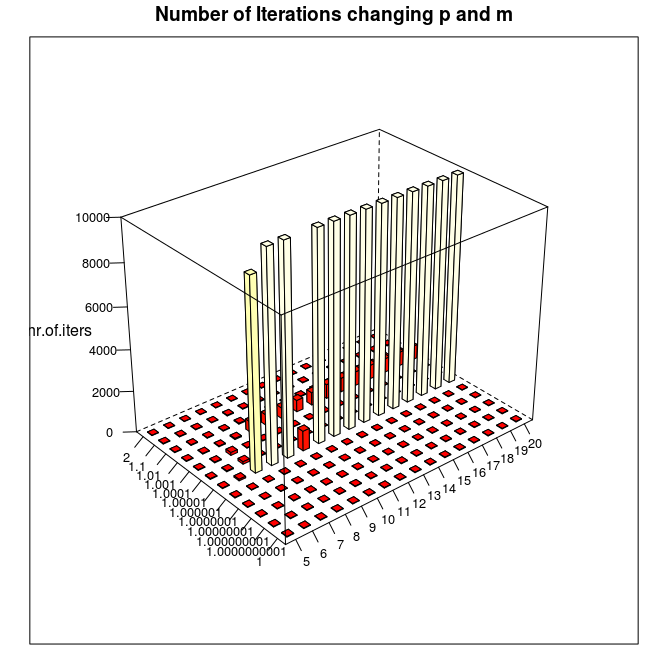
\includegraphics[scale=0.3]{Figures/hist3dmpniter.png}
\end{center}

\begin{equation}
  \begin{aligned}
    f(x_k + \alpha_kp_k) \leq f(x_k) + c_1 \alpha _k p_k^T\nabla f(x_k)
  \end{aligned}
\end{equation}

